\section{Finding Forbidden Structures}

\subsection{Forbidden Structures}

Recall that in the introduction we pointed out that an undirected graph $G = (V,E)$ is an interval graph if and only if it is chordal and has no ATs, which is three vertices $a_1,a_2,a_3$ of a graph $G$ such that they are distinct and there are three paths between each pair of them without using a neighbor of the third vertex and its neighbors. Lekerkerker and Boland derive the forbidden induced subgraphs from this property. We call these subgraphs {\em Lekerkerker-Boland(LB)} subgraphs. 

\begin{theorem}
\cite{lekkerkerker1962representation}
If an undirected graph $G$ is an interval graph if and only if it does not have an induced LB subgraph which is one of the graphs $\rom{1}, \rom{2}, \rom{3}_{n}, \rom{4}_{n}, \rom{5}(n)$ in Figure \ref{lb_subgraph}.
\end{theorem}

In Figure \ref{lb_subgraph}, we can see that $\rom{3}_{n}$ represents the graphs that are not chordal. Other subgraphs in Figure \ref{lb_subgraph} are subgraphs that contains an AT. The double circled vertices are members of the AT.

%\begin{theorem}
%\cite{tucker1972structure}
%A bipartite graph $G = (V_1,V_2,A)$ has a $V_1$-%consecutive arrangement if and only if $V_1$ contains no %ATs of G.
%\end{theorem}

\begin{theorem}
\cite{tucker1972structure}
The (0,1)-matrix $M$ has the consecutive-ones property for rows if and only if no submatrix of $M$ is a member of the configurations of $M_{I_{n}}$, $M_{II_{n}}$, $M_{III_{n}}$, $M_{IV}$, $M_{V}$ in Figure \ref{tucker_matrix}.
\end{theorem}



\subsection{Algorithm for Finding Forbidden Structures}

For designing a certifying recognition algorithm for interval graphs, an interval model can be given to the user to verify if the graph is an interval graph. If the graph fails to be an interval graph, an LB subgraph is an easy-to-check certificate proving the failure. Motivated by the theoretical importance of the LB subgraphs, Lindzey and McConnell\cite{lindzey2016linear} give an algorithm for summarized in Algorithm \ref{TuckerSubmatrix}.

Before we go to the algorithm, we need to introduce a tool for the algorithm. Two rows in the clique matrix overlap if their sets of cliques $A$ and $B$ have properties $A \cap B \neq \emptyset$, $A-B \neq \emptyset$, and $B-A \neq \emptyset$. The overlap graph of the clique matrix is a graph such that has there is a vertex for each row and there is an edge between two vertices if the two rows in the clique matrix overlap. 

\begin{lemma}
\label{overlapbfs}
BFS on the overlap graph of rows of the a consecutive-ones ordered matrix M can be done in $O(size(M))$ time.
\end{lemma}

The BFS of the overlap graph and its variants will be used multiple times in the algorithm. 



\begin{algorithm}[H]

\SetAlgoLined
%\TitleOfAlgo{Lexicographic Breadth-First Search}
%\BlankLine
\caption{TuckerSubmatrix(M)}
\label{TuckerSubmatrix}
\KwData{A matrix M that does not have the consecutive-ones property}
\KwResult{ The rows and columns of a Tucker submatrix}
\Begin
{    
	M = TuckerRows(M,4) 
    
    \uIf{M has $i \le 4$ rows}{
    	// The rows of M are the rows of a Tucker submatrix;
        
        Find the set C of column vectors that make up a Tucker submatrix;
    }
    \uElse{
    	// Every Tucker submatrix of M contains the first five rows of M;
        
        M $\leftarrow$ FindRows(M) 
        
        C $\leftarrow$ FindColumns(M) 
    }
    
    return M[C]
}       
\end{algorithm}

In the TuckerRows function of Algorithm \ref{TuckerSubmatrix} (see Figure \ref{lm_1}). We try to find Tucker matrices with less or equal to four rows, which is $M_{IV}$, $M_{V}$, and other cases for $k \le 4$. Booth and Leuker's algorithm work row by row, updating the PQ-tree, halting when it reaches a row $k$ such that rows $1,...,k$ do not have consecutive-ones property but rows $1,...,k-1$ do have it. The running time is $O(size(M))$, hence $O(|V|+|E|)$ for chordal graphs.

If the matrix does not have the consecutive-ones property, we will reach such a row $k$. Let $M_{1}$ be the submatrix of rows $1,...,k$ and $Z_1$ be row $k$. To show that $M$ does not have consecutive-ones property, it suffices to consider only $M_{1}$. Every Tucker submatrix in $M_{1}$ contains $Z$ since submatrices that do not contain $Z$ have the consecutive-ones property.

Moving $Z_1$ to the beginning does not affect whether the matrix has consecutive-ones property. Call this matrix $M'_1$. We repeat a second time, halting at the first row $k_2$ of $M'_1$ that breaks consecutive-ones property. Let $M_2$ be the rows $1,...,k_2$ of $M'_1$. Note that the first row of $M'_1$ is $Z_1$. We only need to consider $M_2$ to show that $M$ does not have consecutive-ones property. Let $Z_2$ be row $k_2$. Every Tucker submatrix of $M_2$ contains $Z_1$ and $Z_2$.

It is easy to see that after $h$ iterations we have $\{Z_1,Z_2,...,Z_h\}$ in a matrix $M_h$ such that $M_h$ does not have the consecutive-ones property and every Tucker submatrix has $Z_1,Z_2,...,Z_h$. To find the rows of a Tucker submatrix, we may halt on iteration $h$ such that $Z_1,Z_2,...Z_h$ is all the rows of $M_h$ If we use this algorithms to find the rows of a Tucker submatrix, it will be an $O(|V|*|E|)$ algorithm because $h$ is $O(|V|)$. In Algorithm \ref{TuckerSubmatrix}, we only run five iterations see if we find a Tucker submatrix with less or equal to four rows. For larger Tucker submatrices, we use the Proposition \ref{overlapcycle} to find them.

\begin{figure}[H]
\centering
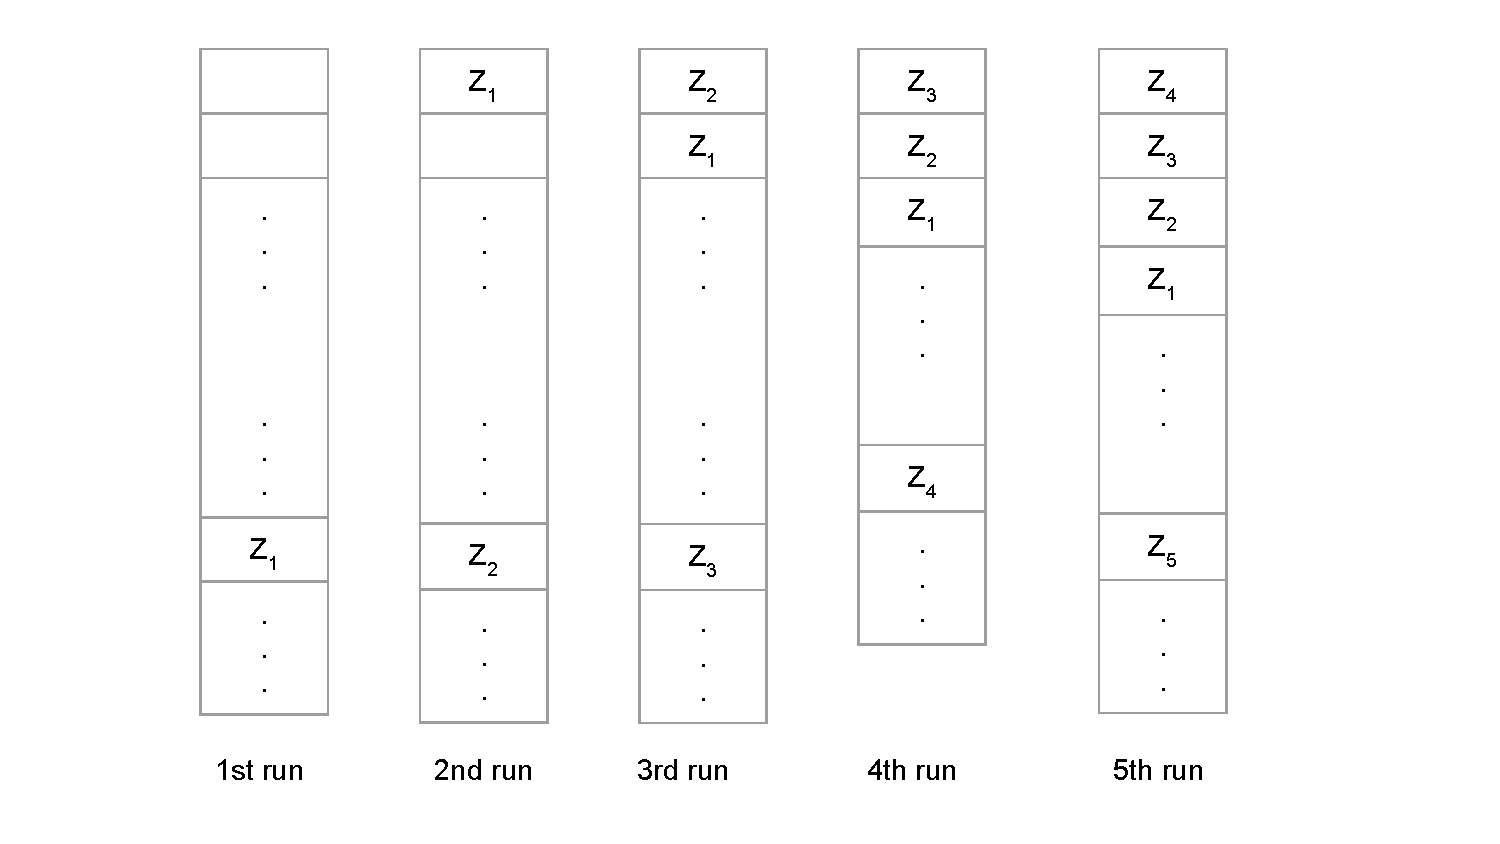
\includegraphics[width=12cm]{figures/lm_1.pdf}
\caption{Steps of TuckerRows function}
\label{lm_1}
\end{figure}

\begin{proposition}
\label{overlapcycle}
The overlap graphs of $M_I{k},M_{II}{k},M_{III}{k}$ are simple cycles.
\end{proposition}

For a cycle in the overlap graph, the rows which are on the cycle must contain a Tucker submatrix. If the cycle we find is minimal, it is a minimal set of rows that contains a Tucker submatrix. 

\begin{definition}
\label{sp}
Let $R'$ be a set of rows of M such that $R'$ has the consecutive-ones property but $R'\cup{Z}$ does not. Rows $A, B \in R'$ are a \emph{suitable pair} for $Z$ if they are members of the same overlap component $R_Q$ of $R'$, each of $A$ and $B$ contains a $1$ of $Z$ and in a consecutive-ones ordering of $R_Q$, a $0$ of $Z$ lies in between $A$ and $B$.
\end{definition}

\begin{figure}[H]
\centering
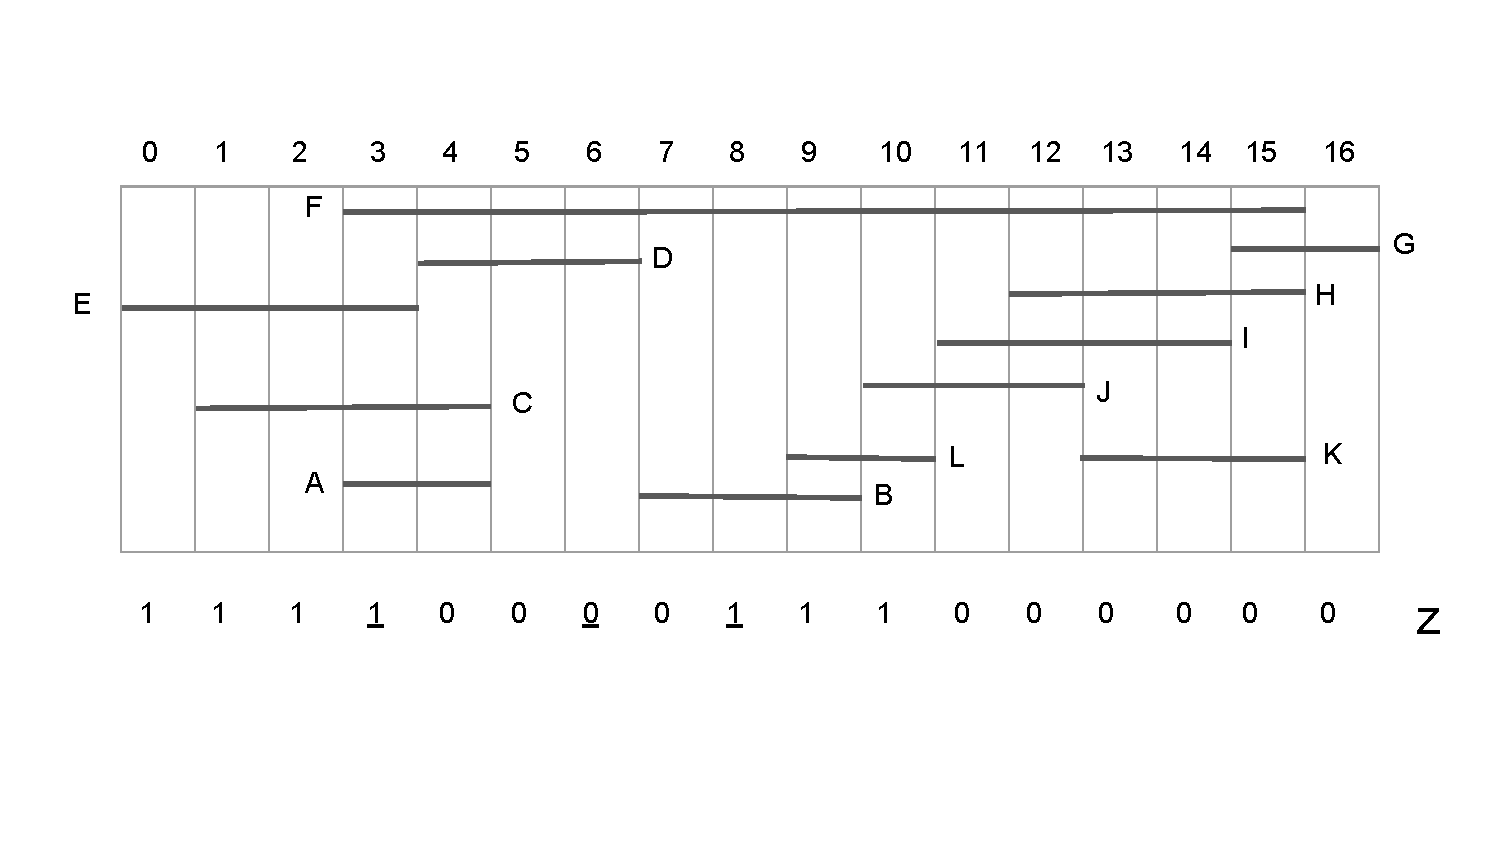
\includegraphics[width=12cm]{figures/lm_2.pdf}
\caption{Example of a suitable pair A and B}
\label{lm_2}
\end{figure}

If after we run function TuckerRows and still cannot find a Tucker matrix that has less or equal than four rows, we know the first four lines of the order must be in a Tucker submatrix. In the fifth run, let $Z$ be the row which we find out the matrix does not have consecutive-ones property anymore. Let rows before $Z$ be $R'$. Since $R'\cup{Z}$ does not have the consecutive-ones property, and its clique matrix has one of $M_I{k}$, $M_{II}{k}$ or $M_{III}{k}$ as submatrix, there must be a cycle in the overlap graph. Since $R'$ has a consecutive-ones ordering while $R'\cup{Z}$ does not, $Z$ has to be in the cycle. The rest of the problem is how to find an irreducible cycle that contains $Z$. 

The strategy is to find a suitable pair {$A$,$B$} and a shortest path $P$ from $A$ to $B$, so that $P$ and $Z$ forms a cycle. To find a suitable pair, each time we let a candidate $Z_i$ to be $Z$, we explore the overlap graph of the consecutive-ones order $M'$ formed by other rows $R'$ except $Z$. For each component in $M'$, we find out the member $A'$ with the leftmost right endpoint among rows that contains a $1$ of $Z$, and the member $B'$ with the rightmost left endpoint among rows that contains a $1$ of $Z$. If a $0$ of $Z$ occurs in between $A'$ and $B'$, we find a suitable pair $A'$ and $B'$ with $Z_i$. $A$ and $B$ are in the same overlap component makes sure such path always exists. It is easy to see that there is a consecutive-ones ordering of an overlap component $R_Q$ forces a $0$ of $Z$ between two $1$'s.

\begin{figure}[H]
\centering
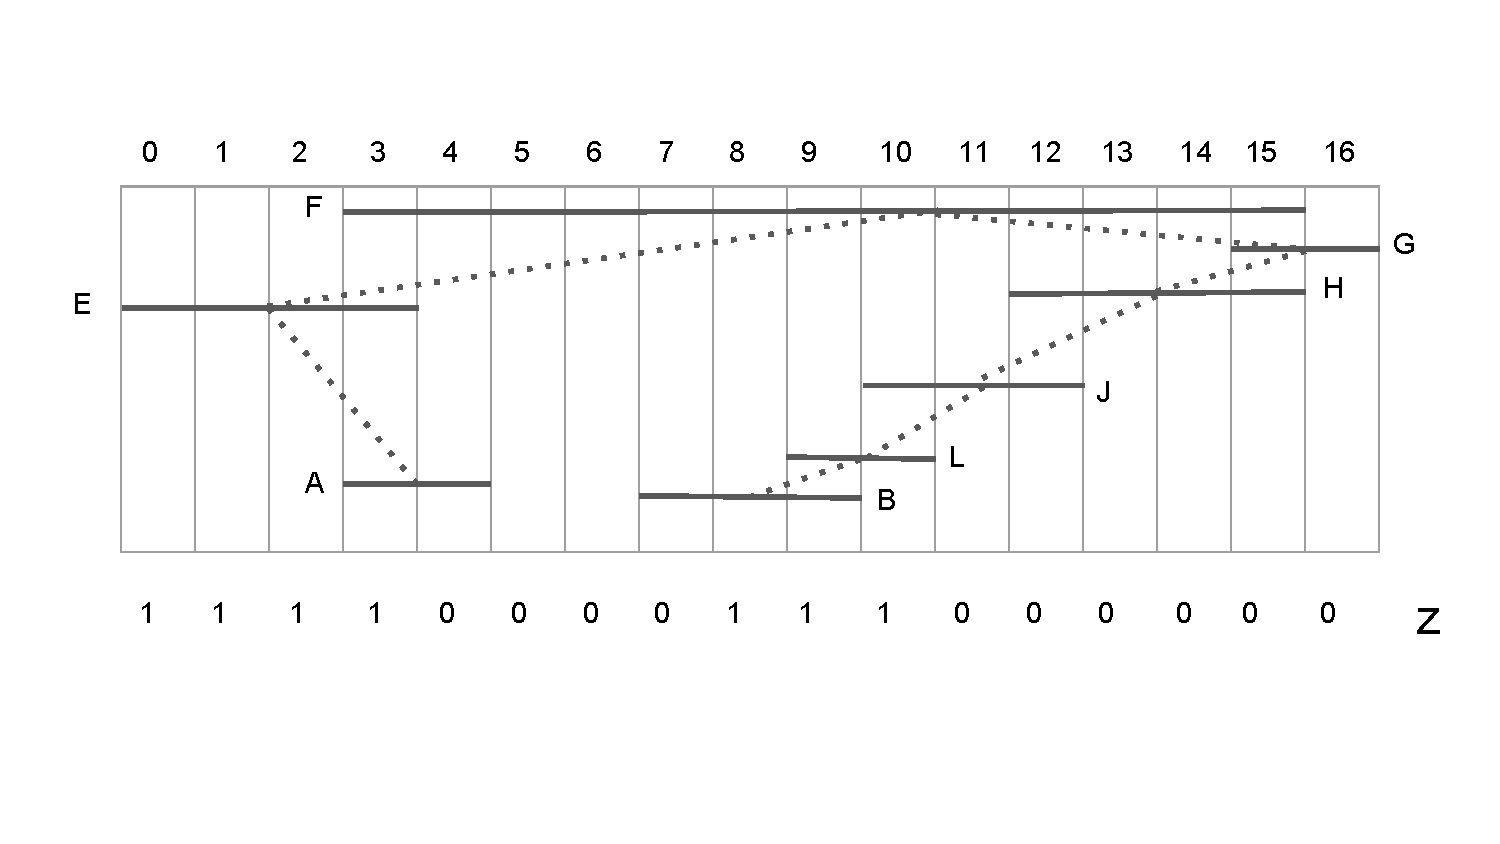
\includegraphics[width=12cm]{figures/lm_3.pdf}
\caption{Example of a shortest path $P$ between suitable pair $A$ and $B$}
\label{lm_3}
\end{figure}

Let $P$ = ($A=R_1$, $R_2$, ..., $R_k=B$) be a shortest path from $A$ to $B$. Since $P$ is a shortest path from $A$ to $B$, then it is an irreducible path, and there are no chords on $P$. However, $P$ and $Z$ may not form an irreducible cycle, a chord including $Z$ may still exist on this cycle. Let $P_1$ = ($Z$, $R_1$, $R_2$, ..., $R_j$) be the minimal prefix of ($Z$, $R_1$, $R_2$, ..., $R_k$) that does not have the consecutive-ones property. Then let $P_2$ = ($Z$, $R_j$, $R_{j-1}$, ..., $R_i$) be the minimal prefix of ($Z$, $R_j$, $R_{j-1}$, ..., $R_1$) that does not have the consecutive-ones property. The steps above consists the $FindRows$ function in Algorithm \ref{TuckerSubmatrix}. After the $FindRows$ function, $P_2$ makes an irreducible cycle in their overlap graph. Therefore, we are able to conclude that all rows in $P_2$ must be the rows of a Tucker submatrix after running $FindRows$.

\begin{figure}[H]
\centering
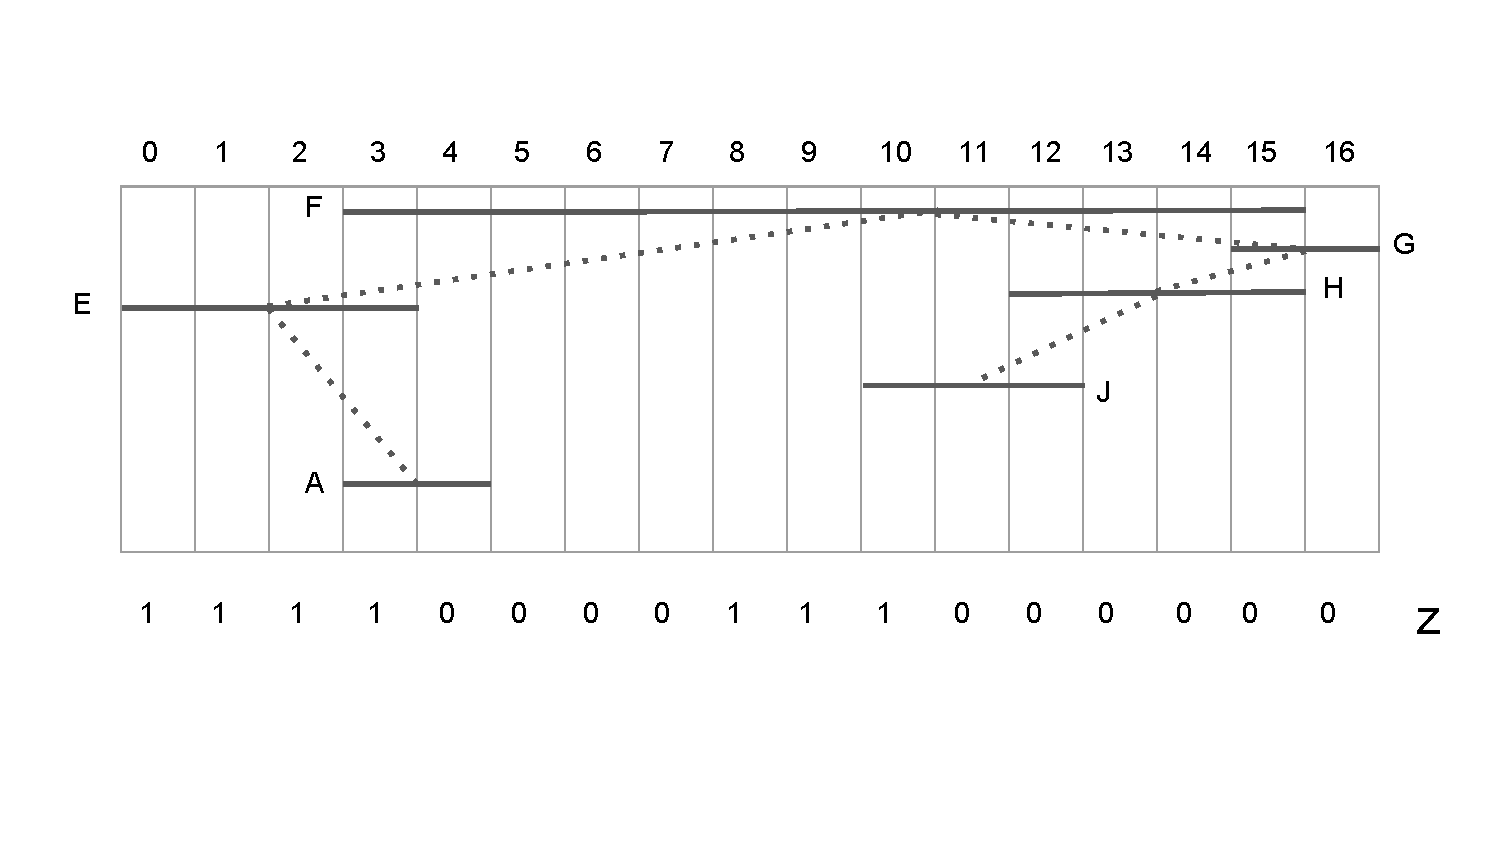
\includegraphics[width=12cm]{figures/lm_4.pdf}
\caption{Example of $P_1$}
\label{lm_4}
\end{figure}

\begin{figure}[H]
\centering
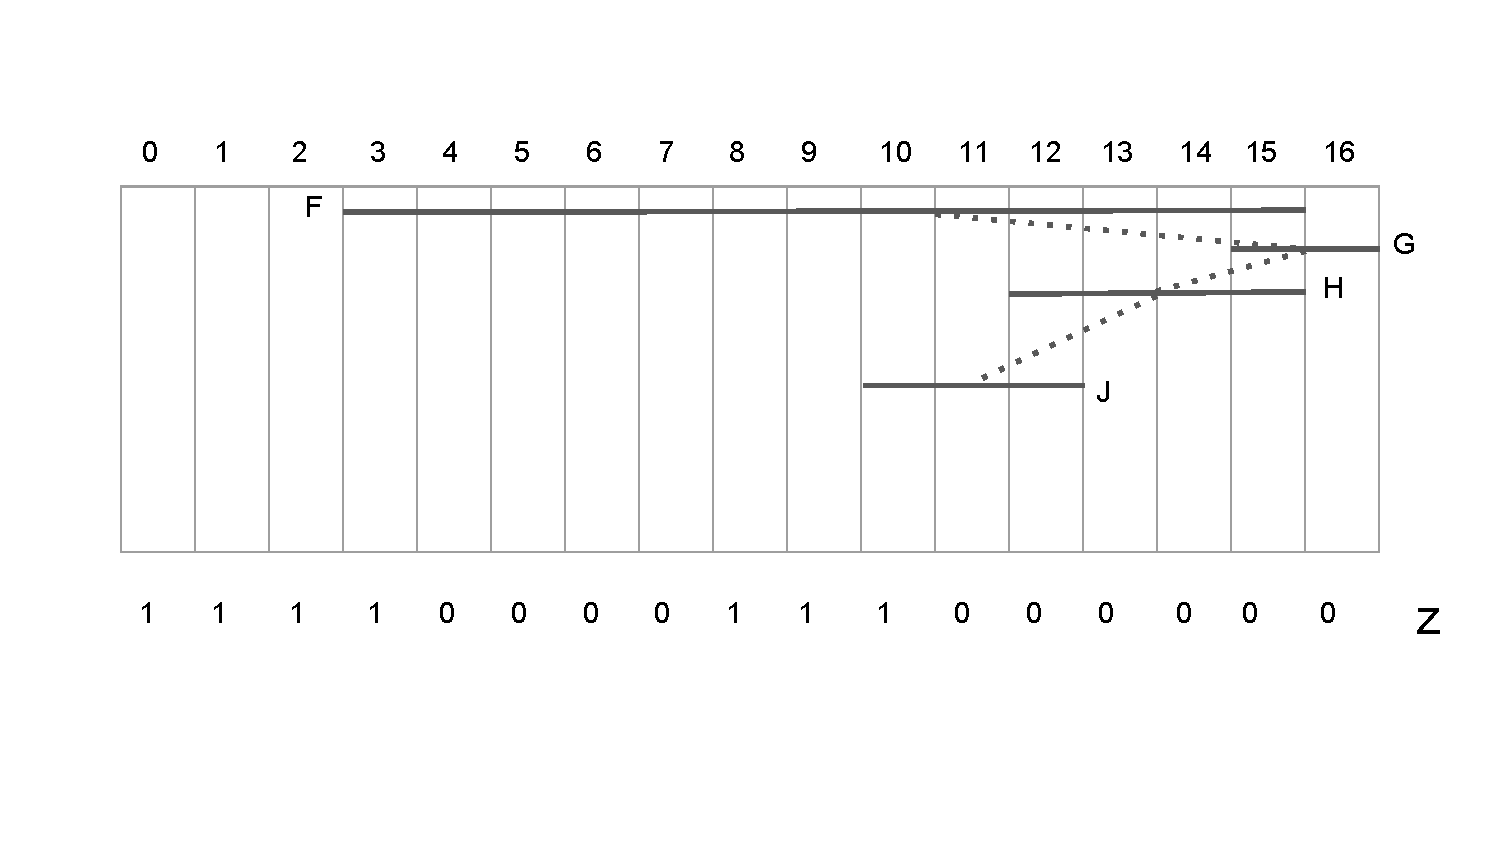
\includegraphics[width=12cm]{figures/lm_5.pdf}
\caption{Example of $P_2$}
\label{lm_5}
\end{figure}

\begin{algorithm}[H]
\SetAlgoLined
\caption{FindLBSubgraph(G)}
\label{findlb}
\KwData{$G$ is not an interval graph}
\KwResult{The vertices of $G$ inducing an LB subgraph.}
\Begin
{    
	Test whether $G$ is chordal using the Algorithm \ref{lexbfs}.
    
    If it is not chordal return an instance of $G_{III}(k)$ for $k \ge 4$.
    
    Otherwise, let M be the clique matrix of G.
    
    Using a call to Algorithm \ref{TuckerSubmatrix} to find a Tucker submatrix $M_T$ in M, let X be its rows in M.
    
    Find three rows {x,y,z} of M that complete $M_T$.
    
    Return $X\cup{x,y,z}$
}       
\end{algorithm}
\begin{lemma}
\cite{lindzey2016linear}
Suppose that $G$ is chordal, $M_T$ is a Tucker submatrix in the clique matrix $M$ of $G$, and the rows of $M_T$ are a minimal set of rows that contains a Tucker submatrix of $M$. Then $M_T$ is not an instance of $M_T$ is not an instance of $M_I(k)$ for $k \ge 4$, and hence it has three incomplete columns. For every choice of rows $x,y,z$ that complete the three incomplete columns of $M_T$, $x,y,z$ and the rows of $M_T$ induce an LB subgraph of $G$.
\end{lemma}

%The relationship between Tucker matrices and LB subgraphs is depicted in FIGURE(TODO). Nevertheless, even if we find a Tucker matrix and its completion, the rows of the Tucker matrix may not form an LB subgraph, an example TODO.


